% -*- root: These.tex -*-

\section{Principes à respecter pour la construction d'une plateforme }
\label{sec:constante_problematique}

%Cette réflexion menant à la construction d'une démarche systématique pour l'évaluation et la construction de modèle de simulation doit certes être mené dans le cadre d'une amélioration de nos pratiques, mais nous avons vu que cet effort n'avait pas pour vocation première l'établissement d'un standard. En effet, la diversité de ces même pratiques rend impossible et réducteur une telle approche. 

% L'impossibilité d'une démarche englobante universelle

Dans la section précédente, un rapide historique a permis de voir quelles limites récurrentes pouvaient expliquer la difficulté de développement des pratiques de validation. Dans cette section, il s'agit d'établir des principes qui prennent à la fois en compte l'analyse précédente, tout en la projetant dans un contexte de recherche plus actuel, marqué par le retour à des critères de scientificité plus stricts, comme en témoigne les récents débats sur la \enquote{reproductibilité}.

\subsection{Le choix d'une plateforme intégrée}
\label{ssec:choix_plateforme_integree}

%merci d'avoir commencé à retravailler ce point. Il me semble qu'il faudrait être plus clair, c'est parfois encore allusif, et durcir la construction initiale: vous partez par exemple de Netlogo, vous dites ce que ça permet et quelles sont les limites par rapport aux exigences de dimension et d'évaluation des modèles vues dans la partie précédente, et donc vous introduisez ensuite la grille des principes qui vous ont guidés dans la construction de votre plateforme

Au travers du chapitre un et deux on a montré que la problématique de mise en oeuvre d'une méthodologie, d'un protocole pour la construction et la validation des modèles de simulation s'inscrivaient en réalité de façon récurrente dans l'historique de la simulation et cela depuis son apparition. 

Plutot que de se lancer dans un difficile et probablement impossible exercice de comparaison pour la formulation de facteurs communs en cause dans la résurgence de cette problématique à différentes périodes, l'auteur de l'étude a préféré poser pour la suite de cette analyse la question d'une tout autre façon. Pourquoi en effet, plus de cinquante ans après les tout premiers usage de la simulation en géographie, et presque quarantes années après que soit posé la question de la nécessité d'outils ou de méthodologies pour aborder ce problème dans ces différentes dimensions, n'existe-t-il toujours pas à ce jour de véritables solutions techniques ?

Jusqu'au années 1980, la dimension limitante des technologies existantes parait évidente. Il suffit de reprendre la liste des arguments pouvant justifier de la baisse de confiance touchant la pratique de la simulation après son introduction dans les différentes disciplines pour comprendre l'attachement de certains facteurs (3, 6, 7, 8) à une dimension technologique limitant fortement la création et l'exploration de modèle de simulation : accès physique et conceptuel aux ressources informatiques disponibles difficile, limitations \textit{hardware} et \textit{software} dans l'expression et l'execution des programmes dédié à l'exploration ou à la création de modèle de simulation, etc.

L\ref{ssec:crise_mutation} nous as permis d'illustrer plus spécifiquement chez les géographes quelqu'une des diverses limitations liés à l'informatique au travers des grandes mutations qui l'ont touchés. On retrouve ainsi chez chez les géographes pionniers anglo-saxons ou européens \autocites[155]{Batty1976}{Openshaw1996}{Pumain, Amoral} divers témoignages qui aborde cette problématique informatique sous l'angle institutionel, ou de façon plus pragmatique dans la tâche de modélisation. 

Ainsi, même si il est déjà possible de projetter sur la réalité une forme d'explication \enquote{curieuse} à partir de modèles à la dimensionalité réduite (Schelling, Lotka-Volterra), les capacité techniques alors disponible contraigne fortement l'expression et le développement de modèle de simulation capable d'assumer une complexification pourtant nécessaire dans le cadre d'un dialogue organisé avec l'empirie. 

 (voir section \ref{ssec:evaluation_construction}).

Si on met de coté les travaux des pionniers américains, la période marquant véritablement l'accès plus généralisé à des outils support de la simulation se situe plus dans le courant des années 1970 que 1960. Les débuts de la micro-informatique, couplé à l'irruption de langage informatique dédié à la simulation fournit le support matériel, accessible, d'une pensée systémique jusque là demeurée très abstraite. 

nous assurent de la difficulté de calibrer les systèmes dynamiques non linéaires sans faire appel à des techniques d'optimisation couteuses, encore très limitées et de mise en place on l'imagine très difficile du point de vue d'un géographe à l'époque. D'un autre coté, l'execution de modèle spatialisé discret s'appuyant déjà sur des formes en réalité plus ou moins hybridés \Anote{note_varenne_hybride} de modèle de simulation  préparant \autocites{Hagerstrand1957, Morril1962, Tobler1970, Allen1978, Wilson?} la diffusion dans les années 1980 du formalisme d'automate cellulaire AC \autocites{Tobler1979, Couclelis1985} \autocite[32-38]{Louail2010} sont également très fortement contrainte par les capacité mémoire des ordinateurs \autocite{Marble1972} et l'absence d'une algorithmique et d'une architecture physique permettant d'accéder au parallélisme nécessaire à la complexification des modèles.

%de modélisations deviennent véritablement disponible ,Les modèles de simulation fournissent dès les années 1970  technique de  systèmes complexes au modélisateur, et cela de façon quasiment conjointe à l'initiation systémique entamé en amont comme on a pu le décrire dans la section xx.

Mais il a fallu attendre la fin des années 1980 et l'invention d'un \textit{hardware} et d'un \textit{software} adapté pour que puisse être observé dans des simulations les comportements émergents guidé par une logique réactive individualisé dans des simulations des fourmillières nécessitant plusieurs milliers de fourmis. On citera par exemple la version parallélisé de Logo réalisé par Resnick et nommé MultiLogo s'executant d'abord sur une Connection Machine spécialisé dans le calcul parallèle, également utilisé pour les travaux de l'équipe de l'équipe de UCLA (RAM, Genesys/Tracker system, AntFarm), et de façon plus générale les premiers essai de plateforme logicielle dédié à l'execution de CA, comme celle de Langton (CellSim), et bien d'autres dont on trouve trace dans les fils de discussions archivés d'Usenet. 

On notera également les travaux de l'équipe francaise d'informaticiens Drogoul et Ferber (inspiré par les travaux de Deneubourg, Steelsn Theraulaz) sur EMF MANTA, développé sur une base ACTALK, une librairie Acteur pour Smalltalk, utilisé pour ses possibilités de parallélisme \hl{ref section avec ajout de ce petit bout d'historique : Jefferson1990, Drogoul1994 p6, interview de Hiebeler, etc. } % Dans drogoul1994, Drogoul1992 il est également fait notion d'une utilisation tourné vers un public non informaticien, (à voir ou on peut caser ca)

% Marrant de voir que Deneubourg en 1989 a fait du monte carlo dans un espace discrétisé en 2D cf "he Blind Leading the Blind: Modeling Chemically Mediated Army Ant Raid Patterns" ... 

% Il y a aussi boids, l'autre partie bio inspirée par le paradigme acteur, et les travaux sur les particules, qui nécessitent surement plus encore de calcul ... Reynolds1987 à trouver...

Malgré la levée progressive de ces différents verrou à partir de la fin des années 1980 (section \ref{sssec:communautes_jasss}), comment se fait il qu'il n'y ai pas eu, parmis les multiples innovations marquant ces trois dernières décennies, une innovation se focalisant plus spécifiquement sur la mise en place d'une solution de validation des modèles de simulation plus systématique et générique ? 

La question qui apparait ici comme volontairement naïve, reflete pourtant ce constat répété et actuel de l'absence d'une telle solution dans la littérature des modèles agents, tout comme elle l'avait été dans la littérature des modèles en système dynamique (section \ref{p:validation_nouveaux_outils}).
%Dans la section validation nouveaux outils il faut se limiter vraiment à la présentation de la problématique de protocole, juste un état des lieux donc pour permettre une présentation plus détaillé des solutions existantes par la suite.

Dans un article publié dans un ouvrage marquant les 20 ans de la publications de \textit{models in geography} \textcite{Openshaw1989} dresse un constat critique des travaux de modélisations théoriques. La citation ci-dessous est tiré de l'introduction d'une catégorie qui nous intéresse particulièrement \textit{A lack of both empirical Validation and Application} 

\foreignquote{english}{[...] But even when data do exist, there has been no systematic and comprehensive attempt to validate existing theories, unlike physics where theories are constantly being tested experimentally. A related difficulty is the lack of any clear idea as to how a model should be evaluated. What criteria can be used to define acceptable levels of performance ? What levels of descriptive, predictive, and forecasting performance are likely to be indicative of a well-performing model?} \autocite[78]{Openshaw1989}

Une remarque à la suite desquel il nomme deux problématiques. L'absence de logiciels d'une part \Anote{point_un_openshaw} est déjà considéré comme problématique au début des années 1990. Déjà difficile à se procurer dans les années 1980, le modèle de Peter Allen l'est probablement encore un peu plus aujourd'hui, si celui n'a pas déjà disparu. Qu'en est il du modèle de Wilson, dont on ne trouve pas une autre description que mathématique ? Et les premiers modèles d'Hagerstrand développé en Fortran par Marble et Pitts ? Un constat qui touche également les constructions plus récentes, ainsi qu'est il advenu du code source du premier modèle agent en géographie \enquote{Simpop}, dont la création ne remonte pourtant qu'à une vingtaine d'année ? Entre d'une part la disparition de code source support des modèles, et d'autres part l'absence de description suffisament élaborées pour repliquer les modèles, comment dans une société dominé par les usages de l'ordinateur peut on maintenir un interet pour une description papier de modèles pourtant historique de par leur inscription spatiale \textbf{Dynamique} et \textbf{Temporelle} !

Sortie de ces considérations qui tiennent plus d'une réflexion sur les travaux d'archéologie digitale qui attendent les futurs géographes, que peut on dire aujourd'hui des modèles ou des logiciels support de la modélisation, sont il disponible ? peut on les utiliser, et si oui, qui en est capable ? Mieux encore, ces logiciels permettent ils de répondre aujourd'hui à cette problématique de l'évaluation des modèles dont on ne finit pas de s'apercevoir à quel point celle-ci est ancienne ?


\Anote{point_deux_openshaw}

Tout comme la seule prise en compte du facteur technologique dans la résolution du problème de l'évaluation n'est pas acceptable, l'attachement de cette problématique de l'évaluation à la seule émergence d'un formalisme informatique est en partie erroné. En admettant comme nous l'avons fait (\href{section}) à l'originalité propre au construction de modèle en géographie, on accède à la construction historique et cumulative d'une boite à outil avant tout au service de la question géographique; l'utilisation et l'imbrication flexible des éléments qui la composent devenant elle-même une forme d'invariant méthodologique qui dépasse la problématique technique. Autrement dit, les problématiques mobilisées lors de la construction d'un modèle de simulation, qu'il soit de type SD, AC ou Agent sont en réalité sensiblement les mêmes. L'observation d'une plus grande pluriformalisation des modèles à même démontré ces dernières années le peu d'intérêt qu'il y'avait à construire des modèles de simulations suivant à la lettre une telle typologie, ce qui n'est pas sans complexifier le travail des épistémologues, alors obligé de décortiquer les formes prises par les hypothèses dans les modèles pour juger de la qualité de leurs relations entretenue avec l'empirie. 



A cela s'ajoute la nécessité pour les géographes d'obtenir des connaissances adaptées qui rendent la plupart des géographes captifs d'un intermédiaire formé pour la manipulation de leur objet de travail. Si cela n'empeche pas la poursuite des travaux de simulation chez un certains nombre de pionniers disposant d'une double compétence, cet aspect va limiter fortement l'inscription et la diffusion des savoirs associés au travers d'une filière universitaire parfois refractaire à ce type d'innovation. 

Ce qui finit de relever ici ce double cercle vicieux dans lequel on s'enferme, car comment peut on inscrire le modèle de simulation comme un outil standard et pérenne de la géographie si d'une part l'apréhension des techniques nécessaires à son utilisation ne figure par ailleurs dans aucune filière universitaire, et d'autre part l'outil peine à convaincre cette même filière par l'absence d'une méthodologie concrete d'évaluation justifiant les connaissances apportées ?    

% ouverture disciplinaire

!!
	Autrement dit, et si on prend pour exemple le point de vue d'un géographe voulant aujourd'hui réaliser son premier modèle de simulation, le fait de savoir que des moyens informatiques tout à fait adéquat existe aujourd'hui pour créer et explorer des modèles de simulation \textbf{n'apporte qu'un faible réconfort si on ne sais pas par où commencer, ni ou l'on va, ni comment on y va.}
!!

Ces arguments, dont on pourrai penser qu'ils sont en partie révolus, on en trouve pourtant une trace substancielle dans l'HDR récente du modélisateur et géographe Arnaud Banos \autocite{Banos2013}. Un témoignage précieux qui donne à la fois la mesure des avancées réalisés, mais constitue également un recueil de prescriptions qui situe très bien les nombreux jalons qu'il faut encore aborder pour parler d'une véritable libération de la modélisation en géographie et en science humaine. \autocite{Banos2013}.

Si il existe bien quelques tentatives de reproduction de ces modèles dans des thèses ou dans des réseau de modélisateurs (le réseau MAPS par exemple, avec le développement de modèles comme Von Thunen, etc.), le travail à faire pour couvrir, redécouvrir et diffuser un support computationel couvrant l'histoire des modèles en géographie parait encore énorme.

En réalité, il faut attendre le début des années 1990 et l'avénement de plateforme adaptés à des non programmeurs, comme StarLogo ou Netlogo, pour que la possibilité d'une autonomisation plus large des géographes vis à vis de leur objet de recherche puissent se généraliser. Nous verrons toutefois par la suite que cette seule possibilité d'accéder à des plateformes plus simple et expressive ne répond qu'à une partie des problèmes. Celle-ci ne traite par exemple ni de l'absence de méthodologie concrete pour la construction des modèles, ni de la problématique d'accès aux ressources informatiques nécessaire à la calibration et l'exploration efficace des modèles de simulation, ce domaine d'expertise restant encore très éloigné du portefeuille de compétence accessible aux géographes.

Il apparait comme urgent de sortir d'un cercle vicieux où les modèles de simulation lorsqu'ils sont construits ne peuvent être que difficilement explorés, calibrés et publiés ! Le défaut de résultats, l'absence d'exploration ou de calibration dans les publications ne font alors qu'alimenter un manque de crédibilité qui ne dessert ni la diffusion, ni l'évolution des pratiques qui pourrait permettre entre autre l'autonomisation des géographes vis à vis des outils informatique manipulés. Si cela n'empeche pas la poursuite des travaux chez un certains nombre de pionniers disposant par chance de compétence multiples, cet aspect va limiter fortement l'inscription et la diffusion des savoirs associés au travers d'une filière universitaire parfois refractaire à ce type d'innovation. Ce qui finit de relever ici le cercle vicieux dans lequel on s'enferme, car comment peut on inscrire le modèle de simulation comme un outil standard et pérenne en géographie si l'apréhension des techniques nécessaires à son utilisation ne figure par ailleurs dans aucune filière universitaire ? 


%C'est en cherchant à savoir quels étaient les motifs de la recurence d'un tel questionnement que sont apparu plusieurs facteurs susceptible d'avoir limité l'émergence de tel outils.

%La section  a montré que malgré la levée de tout ou partie de ce problème, l'absence d'un cadre plus formel supportant de façon satisfaisante les différentes dimensions se rapportant au problème de la validation était toujours d'actualité. Uhrmacher2009 p12

!!
	La mise en perspective de différents points de vue opéré dans la section \ref{ssec:triple_lecture} a permis de rapeller que ce \enquote{problème de la validation} ne pouvait être analysé de façon \textit{top-down} en excluant les spécificités disciplinaires et en se basant sur une lecture de dimension uniquement technique, méthodologique, epistémologique ou philosophique. 
!!

Dans le chapitre 2 et particulièrement dans la partie décomposant l'approche d'Hermann, on a vu qu'il fallait.

%Saisir les composantes de la validation dans une déconstruction de l'activité de modélisation, une activité certes souvent évoquée par les guides méthodologiques mais en réalité rarement mis en oeuvre dans les fait; on l'imagine du fait de la profonde mise en contexte que cette activité impose.

Le chapitre 2 a montré que la charnière des années 1970 avait constitué de façon générale un moment important modifiant la perception que l'on pouvait avoir du problème de la validation. Les apports de Forrester (section \ref{sssec:forrester_impact} et d'Hermann sur cette question de la validation peuvent être mis en perspective d'une discipline géographique opérant déjà en interne l'analyse et la transformation de ces pratiques. 

\hl{ ---- DEBUT EN COURS ---- }

Le modèle qu'il soit informatique ou posé sur papier, reste un construit dont la validation renvoie avant tout à l'évaluation d'un raisonnement. 

\Anotecontent{outil_modification_raisonement}{Alors même qu'il est de plus en plus reconnu que l'outil joue sur la forme et le développement de nos réflexions, le débat reste intéressant à suivre \hl{ref google, ref papier crayon vs ordinateur pour la prise de notes, petite poucettes de M. Serres}}

La transposition à la simulation a permis de développer encore un peu plus loin les formes prises par ce questionnement, en substituant la feuille de papier par un substrat informatique, plus efficace. Or comme le dit très bien Amblard pour répondre au critique des détracteurs de la simulation s'appuyant sur cet argument, on ne pense que très rarement à remettre en cause la feuille de papier comme support de la réflexion \Anote{outil_modification_raisonement}, car ce n'est tout simplement pas ça qui nous intéresse immédiatement. 

, celle de la construction et l'accumulation de sens qu'il est possible en confrontation directe avec une réalité telle qu'on peut la capturer dans nos mesures, dont on sait qu'elles sont toujours critiquable en sciences humaines. 

La plongé dans cette nature contextuelle de la validation révèle alors l'importance de valoriser auprès des pairs cette trajectoire de construction du modèle constitutive du raisonnement, la seule possibilit.

Si la nature et la diversité des outils, leur fréquence d'utilisation, l'ordre de leur utilisation et même l'objectif motivant leur utilisation dans un raisonnement scientifique ne peuvent être effectivement anticipés, il reste dans la deconstruction du raisonnement l'execution d'un questionnement récurent et que se pose d'emblée tout modélisateur débutant ou expérimenté : Quand et comment puis je savoir que le modèle que je suis en train de construire peut être considéré comme satisfaisant ?

%La charnière des années 1970 a montré l'ancienneté des débats . Mais force est de constater en lisant les écrits de la communauté M\&S sur le problème de la validation que c'est bien au prix d'une certaine de-contextualisation que les propos pourtant très actuel d'Hermann ont pu être intégré dans la masse d'un arsenal méthodologique au point de vue très ingénierie.

Une solution est alors d'épouser dans un projet de plateforme hébergeant cette activité non pas les modalités nécessaire la systématisation d'un tel questionnement, mais la plastique informatique nécessaire à la mise en oeuvre de ces modalités. 

Il ne s'agit plus d'imposer, mais d'épouser le contexte, en tenant compte de l'existant thématique, méthodologique, informatique.

%Là encore on comprendra le frein au développement de la modélisation qu'à pu constituer la difficulté de prise en main d'un tel outil, destiné principalement jusque dans les années 1990 aux seuls informaticiens, les seul capable de tels développements. Sans compter la problématique de calibration et d'exploration des modèles nécessitant l'intégration de compétences encore plus étendues., qui demande une formation spécifique qu'à pu constituer l technologique imposé par les formalismes informatiques, qui jusqu'à l'apparition plus récente de logiciels permettant au modélisateur

Le modèle de simulation tant qu'il se définit comme un objet dynamique support d'une activité de recherche (section \ref{p:autre_def_modele}) possède une dimension historique. Rendu public, celui-ci échappe alors à ses créateurs,s'autonomise et développe une histoire dont le succès se mesure à l'aune des trajectoires multiples et transformantes qu'il subit \autocite{Banos2013a}. Ainsi n'a-t-on pas déjà évoqué l'histoire de modèles devenus dans leur discipline des mécanismes de référence, point de départ de toute modélisation : daisyWorld \autocite{Dutreuil2013}, Schelling \autocite {Bulle2005}, Sugarscape, Anasazi, et plus proche de nous, en géographie le coeur commun à la famille des modèles de simulation Simpop. 

L'emploi d'un unique cadre formel capable d'anticiper tout autant la possibilité de cumul et la diversité des objectifs, que celle des pratiques des modélisateurs parait de ce fait difficile sinon impossible à mettre en place.

\hl{ ---- FIN EN COURS ---- }

\subsection{Une analyse critique de la méthodologie moderne POM}

%que sur  celle ci ne doit pas être  relativement peu de méthodologie clef en main qui s'attaque de front à cette problématique, la plupart se bornant seulement à l'établissement de guides de bonne pratiques, ou de listes d'outils (mathématiques, statistiques, informatiques) disponible.

Parmi les tentatives les plus récentes d'approche de ce problème, la méthodologie POM (\textit{Pattern Oriented Modelling}) \autocites{Grimm2005,Grimm2011} proposée en écologie par Grimm et Railsback vient compléter les précédents efforts de standardisation déjà réalisés avec ODD \autocite{Grimm2010}. 

Comme le dit très bien l'auteur dans sa définition de POM \Anote{railsback_POM_resume}, cette stratégie pour la construction de modèle ne fait qu'expliciter une méthodologie la plus souvent déjà opérante chez des scientifiques modélisateurs expérimentés. Toutefois, le transfert de cet implicite dans une méthodologie bien nommée offre au-delà d'un acronyme la possibilité d'une mise en avant de ce processus \enquote{constitutif du modèle} qu'est l'activité de construction (voir \ref{p:autre_def_modele} et le chapitre précédent), une activité pour laquelle on n'accorde encore que peu d'importance dans la construction des publications, souvent au seul profit des résultats. A la différence de la démarche KISS (\textit{Keep It Simple Stupid}), parfois reprise par les auteurs de modèles de simulation comme un argument suffisant pour justifier d'une construction, POM va à mon sens beaucoup plus loin. D'une part, car celle-ci donne à voir un outillage conceptuel beaucoup plus concret pour encadrer, diriger la construction de modèles, et d'autre part, car elle met ce processus en regard de l'élaboration de \textit{patterns}, des critères qualitatifs ou quantitatifs utilisés à la fois comme heuristique pour intégrer des éléments échappant au modèle conceptuel initial, mais également comme filtre permettant de justifier l'organisation interne retenue dans nos constructions. Ainsi, on retrouve dans l'argumentation de Railsback et Grimm cette idée d'élaboration d'une évaluation multi-critères guidée par l'apport cumulatif de crédibilité qu'elle permet sur le réseau d'hypothèses du modèle, un constat déjà esquissé par Hermann à la fin des années 1960 et dont nous avons déjà analysé l'importance dans la section \ref{ssec:evaluation_construction}. 

%10:32 <Skizomeuh> RT @_FabV: [81] Un nouveau long-métrage Ghost in the Shell prévu pour l'été prochain, par l'équipe de ARISE https://t.co/tOnztTF0aA http://t.co/V1SqWwjEZV
% Timur Vermes, un livre énorme ! A lire ab-so-lu-ment !
% RT @GrapheneDB: [52] Popoto.js a graph search generator JS lib for the @neo4j #graphdb, by @FredCiminera - http://t.co/gn85K2kjYG
% http://t.co/5gjkzz8K08

La première étape de POM intitulée \foreignquote{english}{Pattern for model structure} s'appuie sur l'expertise des chercheurs spécialistes du domaine pour établir la partie \foreignquote{english}{Overview} de la feuille de route ODD : identifier l'objectif motivant le modèle, les entités, les variables, les dynamiques, l'enchainement général du programme, les \textit{patterns}, et les critères de mesure pour ces \textit{patterns} que l'on estime nécessaire pour la construction d'un premier modèle \textit{a priori} capable de faire \enquote{émerger} les \textit{patterns} retenus. La selection des \textit{patterns} permet de fixer outre la limite posée par l'établissement d'un modèle conceptuel, une autre limite qui se rapporte celle-ci à la richesse de la structure interne du modèle. L'objectif de ce processus étant de se trouver à l'équilibre dans ce que les écologistes appellent une \enquote{Medawar zone}, calculé comme étant l'optimum entre \enquote{la position la plus avantageuse d'un point de vue des connaissances extraites} (payoff) et sa \enquote{complexité de mise en oeuvre} (difficulty). Il est évident que seul un modèle de simulation opérationel permet de se positionner dans une telle zone. \Anote{railsback_POM_structure}

L'étape suivante invite donc les modélisateurs, si ce n'est pas déjà fait, à construire un premier modèle fonctionnel, même incomplet, afin d'entrer le plus vite possible dans l'étape dite de \foreignquote{english}{theory development} visant l'amélioration incrémentale du modèle.

La \enquote{dé-simplification} ciblé du premier modèle opérationel passe par la formulation d'hypothèse alternatives (\foreignquote{english}{alternative hypotheses} ou \foreignquote{english}{traits}) spécifique des comportements agents (\foreignquote{english}{agents behaviors}) que l'on veut observer dans le modèle. \Anote{agent_grimm} 

La stratégie \enquote{null theories} \Anote{railsback_POM_nulltheories}  consiste à implémenter pour chacun des comportement d'agent amenés à varier par la suite, une version ne faisant appel si possible à aucune théorie particulière, minimisant de fait l'impact interpretatif du modèle initial. En résumé l'objectif est de pouvoir quantifier dans un premier temps et par rapport au critère renseignant l'émergence des \textit{patterns}, quel est le poids interpretatif attribuable à la structure du modèle ainsi mis à nu, puis d'observer dans un deuxième temps, dans l'évolution du modèle et des hypothèses, quel est l'apport exact de chaque nouveau comportement implémenté sur la dynamique générale du modèle.

Pour Grimm, c'est dans cette activité ou les modèles agents endosse pleinement le rôle de \enquote{laboratoire virtuel} que s'exerce véritablement l'activité de raisonnement scientifique. Le modélisateur est amené à exercer son talent de détective via tout les moyens classiques de l'entreprise scientifique, cela dans le but d'imaginer, d'implémenter puis de juger par la mise en concurrence et l'évaluation de paramètres et d'hypothèses alternatives le modèle le plus à même de reproduire les \textit{patterns} retenus jusqu'alors. 

\begin{figure}[h]
\begin{sidecaption}[fortoc]{ POM cycle for developping theory for an agent behavior \autocite[245]{Railsback2012}}[fig:S_syntheseGrim]
  \centering
 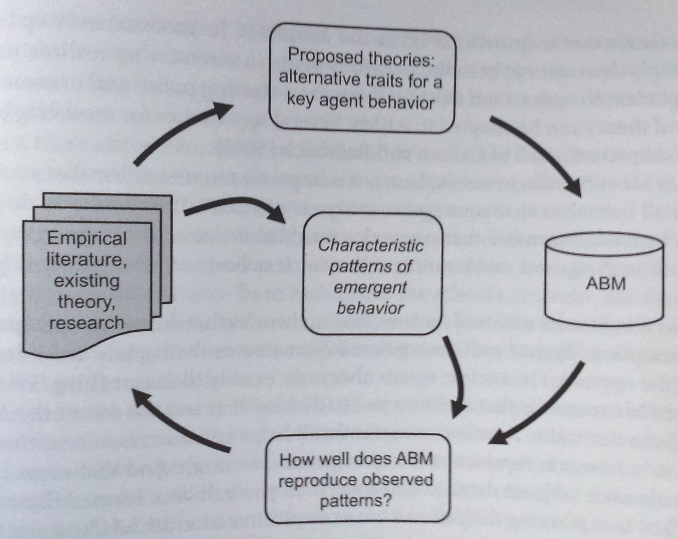
\includegraphics[width=.9\linewidth]{cyclePOMcomportement.png}
  \end{sidecaption}
\end{figure}

Il est tout à fait possible de voir le dialogue qui peut s'instaurer entre ces deux grandes étapes, la structure initiale très simple du modèle s'adaptant progressivement et de façon conséquente aux résultats tirés de l'analyse confrontant \textit{patterns} et données résultats du modèle. Une confrontation dont l'analyse permet de voir émerger non seulement la formulation de nouvelle hypothèses, mais également la modification ou la création de nouveau critères, et patterns. Ce cycle est très bien illustré par la figure \ref{fig:S_syntheseGrim} de Grimm et Railsback.

L'analyse est une étape qui porte la compréhension du modèle, et nous sommes en accord avec Grimm pour dire que celle-ci est indissociable de la construction du modèle, et doit être mis en oeuvre le plus tôt possible, dès que celui-ci s'avère fonctionel. \enquote{Sinon comment justifier de la connaissance produite avec un modèle de simulation ?} Cette question renvoie aux réflexions épistémologiques et philosophiques avancées dans le chapitre précédent. Le fait que le modèle de simulation s'exécute ici sur un substrat artificiel détaché de toute réalité physique est depuis longtemps reconnu comme un des arguments favoris des détracteurs de la simulation. Bien que reconnu comme assez ancien, cet argument montre par sa présence encore aujourd'hui dans l'argumentaire de certains auteurs et certaines disciplines, qu'il est important de montrer à quel point les modélisateurs apportent un soin à faire de ce transfert des conclusions des modèles à la réalité une affaire prudente. % Cf appel réf monde crédible dans le chapitre précédent ?

La qualité, la disponibilité et la reproductibilité du modèle, et du raisonnement qui lui ont donné naissance deviennent alors des pré-requis absolument nécessaires pour parer à toutes critiques concernant la scientificité des résultats apportés par ce type de modélisation. % qu'il s'éloigne finalement assez peu des techniques déjà mis en oeuvre pour la construction de modèle de simulations équationels, .

Car comment peut on faire état d'un transfert possible de connaissance à la réalité si l'étape préalable qui consiste à analyser les comportements du modèle n'est pas réalisée ? Comment justifier de la construction d'un modèle dont on ne mesure pas son fonctionnement interne à l'aune des critères dont on dispose pour caractériser la réalité dont on veut rendre compte ?

L'approche de Grimm et Railsback constitue à bien des égards une véritable avancée pédagogique, de par sa double implication méthodologique et technique et, car elle offre enfin un plan d'attaque lisible pour les débutants, où les objectifs à atteindre sont visibles car explicités par le modélisateur dès le départ. \hl{en cours de reformulation}

Si elle met bien en valeur l'importance de cette activité de raisonnement qu'est la deconstruction, reconstruction des hypothèses du modèle, Grimm oublie il me semble de poser une question importante qui nécessite de rentrer un peu plus dans la processus de construction. % pour la crédibilité d'un raisonnement aussi linéaire dès lors qu'on est confronté à un vaste réseau d'hypothèse.

Comme le décrit Grimm, les \textit{patterns} jouent le rôle de support heuristique accompagnant l'apparition des entités ou des processus que nous n'aurions justement pas pensé à injecter dans le modèle en première analyse. Il est alors évident que ce processus nécessite une grande plasticité dans la formation des hypothèses alternatives, dont le niveau d'abstraction et de formalisation n'est en aucun cas homogène, au contraire. Or Grimm ne dissocie l'hypothèse de sa traduction informatique que sur des exemples très simples. Mais notre expérience acquise en modélisation a montré que la variabilité introduite dans ce processus est double, et peut apparaitre à la fois au niveau de la traduction informatique d'une seule et même hypothèse, tout autant que dans sa formulation alternative. Ces deux interventions peuvent rapidement impacter toute ou parties des éléments déjà mis en places, que cela soit au niveau conceptuel et, ou informatique. On peut pour donner un exemple, se poser la question de la définition des modalités d'un marché régissant les échanges au niveau de chaque ville dans un système de villes pour donner un aperçu de la multiplicité d'hypothèses et d'échelles qui peuvent être envisagées lors de sa traduction informatique, et cela sans compter la combinatoire qui en résulte : définition de la portée des échanges ? stratégies régissants les échanges ? influences environnementales ? etc. Cette hypothèse ouvre, même en restant dans une optique parcimonieuse, vers une multiplicité de sous-modèles et d'hypothèses alternatives dont l'implémentation appelle forcément la création ou la modification d'autres entités et d'autres processus. Autrement dit, il y'a très souvent des incompatibilités et des inter-dépendances qui se forment dans la combinatoire des mécanismes implémentés, l'expansion de cette dernière devenant très vite impossible à gérer si l'on ne dispose pas des outils informatiques adéquats.

Autre point de divergence, la troisième étape de sa posture POM est la paramétrisation et la calibration du modèle. Bien que similaire à la partie développement des hypothèses par le retour sur la structure du modèle qu'il engendre, Grimm justifie l'indépendance de cette étape en évoquant la nature des modifications engendrées, qui ne répondent plus selon lui à une incertitude sur la structure, mais à une incertitude sur les paramètres. Avant de voir pourquoi nous ne sommes pas d'accord avec ce point, il faut faire état des trois définitions qu'il retient pour la calibration. \hl{donner définition}

Lorsqu'elle est rapportée au paramètre (calibrer un paramètre) la calibration \enquote{ is to estimate the value of parameters that we cannot evaluate directly.} Il est relativement courant en science humaine d'avoir affaire à de nombreux paramètres difficiles à calibrer, et cela pour diverses raisons : soit parce qu'une mesure empirique est difficile, voire impossible à obtenir; soit parce que le paramètre représente une valeur agrégée (la translation dans un modèle agents des paramètres alpha, béta du modèle SIR ? ou des paramètres du modèle couplé d'évolution de population de Lotka-Volterra ?); soit parce que les paramètres sont liés à la stochasticité des modèles. Enfin, il faut également compter sur les paramètres qui découlent de l'étape spécifique d'implémentation. Des artefacts nécessaires à l'exécution du modèle (nombre d'objets possibles supportés par le simulateur ? ) peuvent introduire un bruit dont l'influence doit être évaluée régulièrement tout au long de la construction du modèle de simulation.

Ici opère donc une divergence avec l'approche que nous voulons mettre en oeuvre par la suite. En effet pour Grimm, il est d'abord question de mettre en oeuvre une analyse qualitative pour juger de la présence ou de l'absence des patterns, l'analyse quantitative des critères ne venant que par la suite. Si Grimm semble effectivement associer la calibration comme une des étapes à part entière dans sa méthode POM, celle-ci semble se faire avant tout sur des modèles entièrement construits, et ne participe donc pas en elle même à l'évaluation des hypothèses alternatives, opérée en amont. %A REVERIFIER

Dans notre cadre, cette étape est associée dès que possible à la construction du modèle, pour la simple raison qu'il est impossible de quantifier, et même de qualifier la part due d'une hypothèse et des paramètres qui la contrôle une fois celle-ci insérée dans un réseau d'hypothèses au comportement non linéaire... De plus, dès lors qu'on prend en compte la trace temporelle d'une telle activité scientifique, on remarque qu'il est par avance impossible de savoir si une hypothèse choisie pour ses bons résultats en début de construction de modèle n'aurait pas pu être rendue obsolète par une hypothèse alternative à un autre moment de cette construction, car écartée prématurément. Le processus d'évaluation doit donc pour être correct et cumulatif intégrer de façon systématique l'historique des différentes hypothèses alternatives.

Grimm met particulièrement l'accent sur ce que d'autres auteurs appellent \enquote{proof of impossibility} \hl{ref }, un principe inspiré de la démarcation poppérienne; la réfutation d'une hypothèse dans sa capacité à reproduire un ou plusieurs patterns apportant une preuve plus intéressante que sa simple corroboration. Une remarque à mettre bien évidemment en perspective des spécificités propres à la modélisation en sciences sociales, le constat d'une multiplicité d'hypothèses valables possibles amenant l'observation d'un même état final (équifinalité) étant plus analysé en science sociale comme un apport interprétatif dans la lecture des données initiales que comme un véritable défaut rédhibitoire réfutant une théorie générale. 

Il est alors tout à fait envisageable que la combinaison d'hypothèses alternatives qui rendent le mieux compte des \textit{patterns} représentatifs d'un modèle à un instant \textit{t} puisse être amenée à varier à un instant \textit{t + 1}. On a alors plus affaire à une famille de modèles plausibles apportant des réponses différenciées en fonction des \textit{patterns} selectionnés et présentés lors de l'exécution du modèle.

Dès lors, le fait de masquer ou de nier cette activité dans ce qu'elle a de cumulative impute - comme on a pu en discuter dans le chapitre précédent - forcément la part d'évaluation du modèle propre à sa discussion par un collectif d'experts du domaine : la qualité de cheminement du raisonnement menant à la construction du modèle, la non-divulgation de multiples hypothèses testées qui seront peut être retestées en vain par d'autres, la mise en échec d'hypothèses trop vite écartées au vu des mécanismes présents dans le modèle, etc.

%effectivement une méthodologie efficace de construction de modèle, dont on perçoit qu'elle est à bien des égards similaire à celle expérimentée dans notre équipe de modélisation (\hl{cf ref passage Marius dans chap précédent})

%Le passage d'un incrément à un autre se fait par l'injection de critères permettant de garantir la crédibilité du modèle au fur et à mesure que celui-ci se complexifie.

\textit{Sachant cela, est-il possible, compte tenu de cet ensemble de mécanismes, de paramètres de reproduire cet ensemble de critères ? Et si oui, existe-t-il plusieurs combinaisons possibles dans cet ensemble permettant d'obtenir un résultat similaire ?}

On comprend qu'il est très difficile d'isoler par le biais d'une opération manuelle sur le modèle cette fenêtre des comportements permet de répondre à une telle question. 

Grimm sous-entend bien l'opération de complexification que subit le modèle dès lors qu'il participe de cette boucle de développement, mais la question d'une évolution de la grille de critères n'est pas évoquée explicitement. Or la complexification du modèle s'accorde certes avec la multiplication des critères, mais également leurs possibles hiérarchisations et spécialisations. Autrement dit, le plan de construction d'un modèle de simulation parait en réalité difficilement dissociable du plan de construction des critères nécessaires à son évaluation. Les critères mis en place pour évaluer l'adéquation des mécanismes aux \textit{patterns} durant les premières phases de construction doivent être soit différents, soit suffisamment génériques pour rester valables tout au long de la complexification du modèle, ce qui suppose une véritable planification du projet dans le temps.

--- \hl{fin retravail 14/01}

Bien que non rattaché dans l'absolu à un support informatique en particulier, l'auteur s'appuie pour transmettre son message pédagogique sur l'utilisation de Netlogo et de ces outils intégrés pour l'exploration comme le \textit{Behavior Space}.

Si la méthode peut servir à former les jeunes modélisateurs à de bonnes pratiques dans le futur, elle reste contraignante pour qui modélise déjà en suivant sa propre méthodologie. Autrement dit, même si POM est la méthode à suivre quant on débute, je ne pense pas que l'injection forcée d'une méthodologie dans des pratiques de modélisation établies depuis des années suffisent à établir celle-ci. Toute nouvelle approche pour être réussie doit avant tout je pense encapsuler et s'adapter à minima aux pratiques existantes des modélisateurs, tout en leur permettant d'évoluer par la suite si nécessaire. Reste que les modalités d'une telle approche doivent encore être raffinée \textit{Oui mais quelles sont ces pratiques, et qu'est-ce qui dans leur mise en oeuvre empêche une évaluation plus systématique des modèles ? Comment peut-on les faire évoluer sans les imposer de force ?}

, il existe toutefois une dissonance entre la méthodologie proposée et le support informatique véritablement adapté. Si Netlogo est effectivement choisi par les auteurs pour sa valeur d'outil pédagogique, ceux-ci sont, je pense, tout à fait conscients que ce choix ne permet pas en l'état de développer de façon réaliste une calibration basée sur une approche multi-critères dans le cas de modèles plus complexes tels que le laisse supposer POM. \hl{Ajout citation p233 et page 313 et 315}

Autre initiative remarquée, celle menée par l'équipe dirigée par Wilensky connut principalement pour avoir développé le simulateur Netlogo. Parmi les papiers écrit par Wilensky ces dernières années \autocite{Wilensky2007a} plusieurs se rapport à mettre en avant - comme d'autre l'ont fait dans la communauté \hl{ref Epstein, etc}- l'importance de \enquote{pratiquer la reproductibilité} pour nous et pour les autres. Un des objectifs visés étant la constitution d'une communauté scientifique capable de dégager de nouveaux savoirs par le partage et la discussion collective des modèles. Une recette que Wilensky a appliqué avec succès dans la reproduction de nombreux modèles afin de les faire figurer dans sa plate-forme, et qu'il faut évidemment mettre en perspective des principaux traits faisant toute la valeur du simulateur Netlogo. 

Avec Stonedahl \autocites{Stonedahl2011, Stonedahl2011b, Stonedahl2010}, il explore cette fois-ci une autre dimension de la validation en s'attaquant à l'exploration automatique des modèles de simulation écrits en Netlogo. L'outil \textit{Behavior Search} ainsi développé par \textcite{Stonedahl2011a} s'appuie sur des méta-heuristique, principalement de la famille des algorithmes évolutionnaires. Cet outil se place volontairement dans la continuité de l'\enquote{esprit Netlogo}\Anote{stonedahl_netlogo}, à savoir offrir des outils à la fois suffisamment simples d'accès pour s'adapter à un public \enquote{débutant en modélisation}, tout en étant suffisamment complet, évolutif, pour intéresser et accompagner les recherches d'un public essentiellement scientifique. Les outils acquièrent avec leur diffusion à une standardisation qui leur permet de toucher à cette dimension sociale constitutive d'une part de la validation.

L'accroche d'un public aux compétences variables, qu'ils soient experts ou débutants, est un enjeu tout à fait compris par les modélisateurs. La plus ancienne des librairies multi-agents \textit{Swarm} était déjà pensée par Langton comme une étape supplémentaire vers la démocratisation des outils. Un saut qui a permis de fédérer une première communauté, mais qui n'était pas suffisant pour toucher un public de non-programmeurs. Le jumeau scientifique de la plateforme pour enfant StarLogo, Netlogo, a permis ces dernières années de redonner une part d'indépendance aux chercheurs des sciences sociales dans la manipulation de leur objet de recherche \autocite{Banos2013}, cet outil permettant de concrétiser à moindre coût et de façon quasi instinctive le contenu de discussions scientifiques dans un modèle exécutable tangible. Véritable outil d'accompagnement permettant à tout scientifique qui le supporte, de concrétiser et de communiquer une idée au travers d'un modèle dans un temps record. On se rapproche ici d'un système de communication ou le cout d'entrée est très faible par rapport aux gains supposés. 

Mais, si Netlogo répond de façon parfaite à cette nécessité de prototypage rapide et peu couteux, un scénario tout à fait adapté pour découvrir la modélisation; il ne permet pas par contre de répondre à un scénario pourtant classique rencontré par les modélisateurs souhaitant faire évoluer leur modèle sur le temps long au-delà d'une certaine complexité. Ainsi, tant d'un point de vue algorithmique, que du point de vue des ressources informatiques nécessaires à l'exécution et à l'évaluation de modèles, Netlogo ne permet pas de supporter une montée en complexité pourtant naturelle dans le cadre de tels projets. 

On sait également que la diversité et la complémentarité des approches sont un point central dans l'étude des systèmes complexes; or si Netlogo donne effectivement à voir cette diversité par la présence d'une large bibliothèque de modèles, celle-ci n'est abordé que dans une seule dimension, celle du modèle, et sous un seul format, celui de Netlogo. C'est il me semble le désavantage difficile à éviter de tout approches visant une forme de standardisation. Or chacune des disciplines dispose de ses propres outils, de ses propres formalismes, de ses propres formats que Netlogo serait bien en peine de vouloir reproduire à l'identique. Cette diversité d'approche caractéristique des systèmes complexes dépasse qui plus est largement largement le cadre de la seule description du modèle et touche également l'environnement qui peuvent graviter autour de lui. Choisir Netlogo c'est prendre le parti d'un formalisme qui donne accès à une communauté, à un ensemble d'outils, mais qui ne permet pas d'exploiter au mieux les apports de diversités propre aux pratiques de modélisation de chacune des disciplines. 

Au travers de ces deux exemples, on a mis en valeur quelques points d'accroches montrant la difficulté qu'il y a à établir un cadre plus ou moins formel et englobant capable d'articuler l'ensemble des problématiques se rapportant à l'évaluation et à la construction de modèle de simulation.  


L'accès à l'outil informatique pour la construction est en voie de démocratisation, comme en témoigne de nombreux indicateurs, tant sociologiques extérieurs (génération petite poucette de Michel Serres), que politique (programmation de formation américain), qui s'exprime par le développement et la démocratisation de plateforme de programmation accessible à tous : Scratch, Blocky, Vixle (https://www.kickstarter.com/projects/realityfoil/vixle-a-game-engine-for-everyone)
Un support qui maintenant date des premiers travaux du MIT avec Logo/StarLogo ... etc

%  se présente par un ensembles de couplage entre des outils conçu sur une base autonome et standard;

\hl{--en cours--}

Autrement dit, ce projet s'inscrit dans un objectif double, il s'agit à la fois de garantir l'indépendance et la réutilisation des outils dans de multiples configurations, tout en problématisant leur utilisation dans des constructions méthodologique (ou cas d'utilisation) que nous jugeont pertinent pour l'exploration et la construction de modèles en géographie. De ce fait ils participent à l'évolution d'une plateforme appropriable par tout les points de vues, non réducteur car flexible dans le cadre de nos pratiques, et appuyant en plusieurs points cette dimension collective pour la construction et l'évaluation de modèle.
% Construction = Evaluation 

Moto : \enquote{Si je ne peux pas évaluer le modèle à ta place, je peux par contre te donner les meilleurs outils pour que tu puisse le faire} 
= en te donnant les moyen d'etre autonome cad
= en te donnant les moyens de mutualiser
= en te donnant les moyens de t'informer 
Deux axes qui recoupent : reproductibilité (pour moi, pour les autres) , flexibilité (pour moi, pour les autres), puissant ( pour moi, dans l'échange), dynamique (pour moi, pour l'échange)

But a atteindre, 
> utilisation inter-disciplinaire, 
> ouverte aux débutant, ouvertes aux experts
> standardisation interne à minima, externe si l'outil est amené à se développer.
=> Plateforme intégrative 


\paragraph{Un outil de \textbf{construction} et d'\textbf{exploration} de modèle}

D'un point de vue utilisateur, on peut considérer l'existence d'au moins deux modes d'exploration auquel on attribue des objectifs très différents. L'exploration dite \enquote{immédiate} permet de controler et de visualiser le comportement du modèle de simulation en temps réel via l'utilisation des outils mis à disposition par le simulateur support du modèle de simulation. On pense par exemple aux \enquote{moniteurs} et autres \enquote{plot} temps réels mis à disposition de l'utilisateur dans le simulateur Netlogo. 

Si ce mode d'exploration peut être apparaitre dans un premier temps comme un moyen de vérification adapté, la complexification progressive du modèle va mettre très rapidement l'opérateur humain en difficulté. Le comportement non-linéaire typique des modèles de simulation en système complexe ne permet pas d'envisager une exploration manuelle exhaustive des comportements; on peut citer plusieurs raisons à cela. En effet l'opérateur va voir son expertise rapidement mise en cause par l'ajout cumulatif de mécanismes, et paramètres induisant des effets imprévisibles dans la dynamique du modèle. Avec pour conséquence immédiate de masquer les défauts de conceptions, qu'ils concernent le 

 vérification superficielle et très rapide du bon fonctionnement général du modèle, que cela d'un point de vue informatique (absence de bug), ou du point de vue conceptuel. 

Un autre niveau d'exploration consiste à analyser à posteriori les données obtenues sorties de simulation, l'objectif n'étant plus le controle cartographier par le biais d'outils adaptés les comportements en sortie de tout modèle de simulation de type agent. 

Dans un premier scénario, le \enquote{modèle} et \enquote{l'exploration de modèles} sont considérés dans un  comme deux objets indépendants, c'est à dire dont le développement peut tout à fait être dissociés. Le choix fait ici d'un couplage faible entre les deux objets d'études permet de garantir l'indépendance du modèle de simulation vis à vis de l'exploration, et inversement. Il en résulte une forme de généricité qui permet d'envisager l'application de tout type d'exploration envers tout type de modèle de simulation, c'est un premier point fort de la plateforme, un coût d'entrée qui se veut minimum pour l'utilisateur, quelque soit l'état d'avancement de son modèle de simulation.

Dans un deuxième scénario, plus dynamique, la plateforme est utilisé comme support à la création du modèle de simulation. On s'interesse alors au dialogue entre 

L'activité de modélisation mobilise un dialogue étroit entre le modèle et ces deux modes d'explorations. Toutefois, on estime que le deuxième mode est le seul qui permette à l'heure actuelle une évaluation des modèles satisfaisante aux yeux des critères scientifiques. Un point détaillé par la suite. \hl{(pourquoi ? )}

De ce dialogue entre modèle de simulation et exploration du modèle nait l'activité de modélisation, la seule qui puisse ici déboucher sur un modèle évalué.

Cette activité de dialogue entraine une relation de dépendance temporaire entre ces objets, qui permet à la fois d'envisager l'amélioration du modèle de simulation au vu des connaissances acquises dans l'exploration, mais également d'envisager l'amélioration, la standardisation ou la spécialisation des méthodes d'exploration au vu des résultats retournés. 

 selon que l'on veut développer de nouvelles méthodes d'analyses . qui une fois mobilisés dans l'activité de modélisation 

\paragraph{Le support de niveau de dialogues différents}

Dans les modes opératoires de construction de modèle, deux \enquote{moments} théoriques (dans le sens ou guidés par des objectifs différents : 

a) Réduire le temps entre l'implémentation de deux prototypes, se rapprocher le plus possible d'une expérience de pensée qui peut être partagé rapidement. Les outils se font le prolongement d'une discussion scientifique, et privilégie donc une prise de controle rapide et facilement partageable (aprentissage aisé, immédiateté d'implémentation et d'execution, support visuel fort pour la discussion).

Un bon exemple de logiciel adaptés à cette utilisation est Netlogo.

b) Réduire le temps d'execution du modèle pour accélérer l'exploration du modèle : 

Contrainte identifié : perte de controle sur le modèle lié à la nécessité d'intermédiaire => tout le monde ne dispose pas d'équipe inter-disciplinaire sous la main.

Objectif : Pour le moment il n'existe pas vraiment d'intermédiaire efficace sur les deux plan permettant une transition aisé (relogo ?), pourtant l'expérimentation nécessite rapidement un accès à une ressource informatique importante, il est donc important de pouvoir découpler ces modes opératoires de l'utilisation effective des expérimentations.

--
%FIXME : Est ce que les points sont hierarchiques ou pas ? 

En admettant que la démarche de construction de modèle soit équivalent à son exploration des modèles autour du principe d'évaluation, l'évaluation devient un élément indissociable de notre démarche de construction des modèles, impose pour être réalisé la mise en oeuvre et le respect d'un certain nombre de principes que la recherche est censé organiser : Collectif, Dynamique, Flexible, Puissance, Reproductibilité, Extensibilité. 

\paragraph{1 - Collectif}

> Cas d'analyse de plateforme ayant réussi cette transformation en communauté dans le domaine de la modélisation : Netlogo.

L'ouverture au collectif est la première des conditions de réalisation de notre plateforme, car c'est uniquement celle ci qui permet d'envisager à terme une standardisation des pratiques chez les géographes modélisateurs. % on se base sur les exemples existants, de plateforme intégrés.

La capacité à pouvoir échanger, et donc à faciliter les échanges avec les autres scientifiques apparait comme la règle minimum à respecter dès lors qu'on accepte de voir le processus de construction et d'évaluation des modèles à cheval entre objectivité scientifique et résultat d'un processus social. 

Par collectif, on entend cette discussion à la fois interne lorsqu'il s'agit de construire l'expérience dans le cadre des pratiques du laboratoire, mais aussi discussion externe, celle qui échappe en partie aux créateurs du modèle, dès lors qu'il s'agit d'afficher et de confronter l'expérience aux yeux des pratiques extérieures.

On entend également la capacité à acceuillir des niveaux de discours différents, qui vont de l'utilisateur débutants à l'utilisateur expérimentés.

Objectif : Définir une plateforme permettant de supporter dans un premier temps, et de catalyser dans un deuxième temps, cette discussion collective, en usant d'outils adaptés. 

% Voir le contenu du modèle (janet)
% Voir le contenu de l'expérimentation (open mole)

\paragraph{2 - Dynamique}

La construction et l'experimentation autour du modèle sont des activités toutes deux incrémentales, ce qui suppose d'organiser les aspects collectif autour 

Nous avons vu dans la section précédente que le modèle de simulation et le groupe d'expérimentations caractérisant ce modèle sont tout deux des objets résultat d'une activité de recherche opérant dans un dialogue mutuel, et dont le contenu initial est connu mais pas forcément le contenu final.

% nottament dans le cadre des systèmes complexes, ou il n'y a pas d'ensemble finis d'indicateurs mobilisable pour borner notre recherche.

Ces choix qui touchent l'ensemble de ces catégories sont étalés dans un temps qui est celui de la construction du modèle, qui ne peut en aucun cas se résumer à un produit final. 

Objectif : Définir une plateforme permettant de supporter par des outils adaptés une discussion collective focalisé en tout temps et pour tout objet intervenant dans la constitution de cette expérience. Le terme supporter renvoie ici tout autant à la présentation, à l'execution, et à l'échange de l'expérience.

\paragraph{3 - Flexible}

La flexibilité est induite des demandes du collectif, interne ou externe.

La trajectoire d'une expérience se définit dans ces deux cas à la convergence de multiples prises de décisions dont la principale influence est le ou les champs scientifique d'application visés par les modélisateurs : choix d'une question déterminé par le champs scientifique, d'un sous ensemble de mécanismes choisis pour répondre à cette question, d'un sous ensemble de formalismes et de niveau d'abstraction hétérogènes, d'un sous groupe d'indicateurs choisis pour mettre en valeur des résultats amenant une réponse à cette question, et d'expérimentations choisis pour évaluer le comportement du modèle fonction de ces derniers indicateurs. 

Le modèle étant mobilisé pour des fonctions épistémiques qui bien souvent se recoupent, aucune de ces catégories n'echappe lors de l'activité de construction à une forme de redéfinition caractéristique de la dynamique de construction. 

Que cela soit dans une trajectoire d'évolution prévue ou imprévue, tout ou partie des constituants de ces catégories sont amenés à être révisé fonction des axes sur lequel le modèle est amené à se déplacer : déplacement sur un axe disciplinaire, déplacement sur une échelle géographique différente, déplacement sur une échelle de complexité pour la représentation du système cible, etc.

Objectif : Définir un outil permettant de supporter une discussion collective en tout temps et pour tout objet intervenant dans la constitution de cette expérience. 

\paragraph{4 - Puissance}

Ce point fait écho aux limitations d'une part d'accès à la ressource informatique brute (existence d'une ressource), d'autre part aux contraintes liés à son utilisation effective (couplage entre expérience et puissance disponible)

L'accès à une ressource informatique doit à tout moment être en phase avec le développement de l'expérience, hors celle ci connait des modes d'expression différents qui oblige à penser un découplage entre modélisation et expérimentation.

L'accès à des ressources informatiques, compatible avec une utilisation collective, dynamique, et supportant l'enrichissement en tout point

(4 - 1) L'accès facilité à la ressource, quelque soit le public cible
(4 - 2) le niveau d'avancement de l'expérience,
(4 - 3/5) les composants qui constituent l'expérience,
(4 - 6) avec la garantie de pouvoir remobiliser cette ressource 


\paragraph{5 - Extensibilité}

La possibilité pour les scientifiques de prendre en main leur outils tout en garantissant l'intégrité de l'ensemble des points précédents.


> Cas d'utilisation en général de la boucle vertueuse entre outils et standardisation d'outils : GeoDA, analyse stat

\paragraph{6 - Reproductibilité}

La reproductibilité \autocite{Sandve2013} d'une expérience et de son empreinte temporelle induit la possibilité pour le collectif de rejouer l'ensemble des étapes ayant menés à la construction de l'expérience, ce qui suppose le versionnement de l'ensemble des constituants de la démarche, du support technique au résultats, en tenant compte des contraintes imposés par les points précédents.

(6 - 1) suppose la mise à disposition du collectif de cette empreinte temporelle, ou d'un instatané de cette empreinte temporelle
(6 - 2) suppose la possibilité de rejouer la trajectoire et 
(6 - 3) suppose la possibilité de repartir de n'importe lequel des embranchements, et de modifier un ou plusieurs des composants pour éventuellement le republier (6 - 1)
(6 - 4) suppose la possibilité d'accéder à une puissance de calcul supposé compatible avec l'expérience
(6 - 5) suppose la possibilité d'ajouter des composants à l'expérience en tout temps

Le support d'un tel point est évident l'objet d'un énorme travail sur la plateforme.


--

a) La reproductibilité des expériences suppose 

a) De maintenir le lien entre un instantané d'un modèle et les expérimentations associés, b) De posséder l'ensemble des versions des modèles et l'ensemble des versions des expérimentations associés

Le couplage entre les deux reproductibilité induit la possibilité de reproduire les résultats de toute expériences, en tout temps et pose évidemment des question techniques importantes.

Difficile à décrire de façon générale ces grand concepts doivent être projeté sur nos pratiques de construction des modèles pour correspondre à une réalité opérationelle.

--

Dans un premier temps, et pour correspondre à un état de pratique tel qu'il est le plus souvent décrit dans la littérature, deux groupes d'activité ont été isolé. L'activité de modélisation d'une part, qui comprend l'ensemble des activité nécessaire à la construction des modèles, et d'autre part l'activité d'expérimentation qui comprend l'ensemble des activités pour évaluer les modèles ainsi construit. 

%L'expérimentation, tel que décrite par {Amblard2003} et reprise sur une idée de {Wagner} constitue un mode de production de connaissance dont la mise en œuvre est motivé pour la construction et l'exploration du modèle. Par « mode de production de connaissance », il faut comprendre qu'il existe plusieurs façon de produire une connaissance permettant l'évaluation du modèle, c'est à dire sa construction : techniques d'analyses de sensibilités, algorithme génétiques pour le calibrage des paramètres, plan d'expérience, etc. 

%L'évaluation des modèles, qui consiste en une accumulation de ces différentes phases d'experimentation guidé par l'objectif d'une meilleur compréhension du modèle, doit devenir un autre objet que le processus linéaire tel qu'il est souvent décrit, avec un début et une fin.

Nous verrons que ce cadre d'analyse ou les deux activités sont amenés à dialoguer pour la bonne construction du modèle est amené à évoluer par la suite, pour concrétiser le passage d'une évaluation des modèles linéaire à une évaluation des modèles non linéaire qui se rapproche plus de l'activité réelle de modélisation.

Le modèle est un produit résultat d'une activité de recherche à un instant t, et qui une fois mis à disposition d'une communauté scientifique, devient objet autonome dont la trajectoire bien qu'impossible à déterminer, doit être envisagé par des outils d'accompagnement permettant de catalyser et de formaliser les discussions.

Autonomie révèle la modélisation comme une expérience résultat d'une activité de recherche

Les modèles de Schelling, Sugarscape, Anazasi sont des exemples de modèles ayant étés repris, discutés de multiples fois. 

Autant de thématiques remisent à l'ordre du jour depuis quelques années du fait de scandale touchant aussi bien les sciences naturelles que les sciences sociales \autocite{OpenScience2012}. 

Cela sans compter la problématique de sauvegarde \autocite{Vines2013} \autocite{Turner2013} et de mise à disposition pour reproduction des expérimentations réalisés sur les données, les modèles et les expérimentations autour des modèles. Une problématique qui dépasse largement le cadre des sciences humaines et sociales et touche l'ensemble des sciences, et plus particulièrement la biologie. 

Cette remarque vaut dans l'ensemble des sciences, dont on prend conscience depuis quelques années du retard sur la question, des sciences naturelles \footnote{Voir le numéro spécial de \href{http://www.nature.com/nature/focus/reproducibility/index.html}{@Nature} en biologie} jusqu'à la psychologie, les  en avance sur la question car durement touché par des scandales ces dernières années \autocite{Steen2011}, mais aussi en modélisation en science sociale, ou la question est abordé depuis de nombreuses années via des groupes de travail et des publications \autocite{Hales2003} \autocite{Rouchier2013}.

De nombreux outils et guides méthodologiques \autocite{Prlic2012} \autocite{Bourne2013} \autocite{Goodman2014} \autocite{Sandve2013} sont en train de voir le jour pour assurer ces aspects de reproductibilité (regroupé le plus souvent sous le label \textbf{openScience} \footnote{Des fédérations tels que \href{http://opensciencefederation.com/}{openScienceFederation} ont récemment vu le jour, on peut suivre les actualités sur le sujet sur twitter \href{https://twitter.com/openscience}{@openScience}}), tant au niveau des plateformes de publication de modèles 
\footnote{\href{http://www.openabm.org/}{@openABM} \href{http://modelingcommons.org}{@modelingCommons}}, de revues 
\footnote{\href{http://www.nature.com/scientificdata/about/}{@Nature} \href{http://www.elsevier.com/physical-sciences/computer-science/executable-papers}{@Elsevier} et en géographie \href{http://cybergeo.revues.org/}{@Cybergéo}}, généraliste 
\footnote{On notera \href{https://authorea.com/}{@Authorea} \href{http://figshare.com/}{@figShare} \href{http://www.activepapers.org/}{@ActivePapers} \href{http://datadryad.org/}{@dataDryad} \href{http://http://thedata.org/}{@dataVerse} \href{http://www.runmycode.org/}{@runMyCode} \href{http://zenodo.org/}{@Zenodo}}, qu'au niveau des plateforme outils support de modélisation 
\footnote{\href{http://www.openmole.org/}{@openMole} \href{http://www.taverna.org.uk/}{@Taverna} \href{https://kepler-project.org/}{@Kepler} \href{http://galaxyproject.org/}{Galaxy}} ou de protocoles 
\footnote{\href{http://www.protocols.io/}{@Protocols.io} \href{https://www.hivebench.com/}{@HiveBench} \href{http://www.nature.com/protocolexchange}{@Nature}}. 



%A ce sujet, il existe une histoire drôle chez les informaticiens, qui peuvent être régulièrement confronté à des états de l'art comportant pléthore d'approches (méthodologique ou technique) pour la résolution d'un même problème. Ainsi l'informaticien zélé, acteur de notre histoire, allume son ordinateur en arrivant dans son laboratoire et part à la recherche d'une solution pour son problème du moment. Mécontent de ne pas trouver un outil satisfaisant pour son problème à la fin de sa journée, celui ci se dit alors dans un éclair de lucidité " Tentons de créer une nouvelle méthodologie pour unifier toute ces approches hétérogènes en une seule !". Ce n'est que quelques mois plus tard, et au terme d'un développement difficile mais enrichissant, que la solution prend finalement forme. A ce moment là, force est de constater que ce ne sont plus 14 mais 15 solutions concurrentes qui s'affronte alors sur le marché des méthodologies pour la résolution de ce problème. Moralité ? Projeter la construction d'une n-ème méthodologie dans une volonté unificatrice (et donc forcément réductrice) peut certes être un exercice constructif (le protocole ODD qui tente d'unifier la description des modèles est en ce sens une expérience intéressante), mais force est de constater que celui ci a peu de chance d'enclencher le processus de standardisation tant attendu, d'autant plus lorsque cet effort s'exerce dans un cadre largement inter-disciplinaire dont les frontières tant sur les aspects méthodologiques que techniques ne peuvent pas être imaginé/intégré par une seule et même personne.

Sur ce dernier point, une première réflexion révélatrice de cette expérience a ainsi été mené par Thomas Louail et Sébastien Rey au laboratoire Géographie-Cités en 2010 \autocite{Louail2010}. L'objectif de ce travail était de lever les limites des méthodologies et outils existants autour des modèles de la famille de modèle Simpop2 afin d'infléchir une réflexion et des premiers outils prototype pour la construction et l'évaluation automatisé de modèle dans le cadre d'une utilisation collective. Si ce projet a permis de fonder la base d'une réflexion plus large qui nous motive encore aujourd'hui dans la présentation de ce projet, force est de constater que l'ampleur de la tâche une fois décrite rendait difficilement réalisable sa concrétisation en dehors d'une équipe pluri-disciplinaire, mobilisé sur plusieurs années sur ce sujet.

%Bharathy2010

\subsection{D'une démarche systématique à une démarche intégrée}


Deux niveaux de discussion doivent être envisagé, le modèle d'une part, et l'exploration de ce modèles d'autres part.

%Une réflexion en terme d'outils, une réflexion en terme de couplage entre les outils, une réflexion en terme de plateforme support garantissant une dimension collective à cette réflexion.

L'objectif est la mise en place d'un outil qui fait office d'attracteur,  capable d'intégrer des outils et des méthodes, mais aussi d'incubateur capable de catalyser un processus de standardisation des outils ou méthodes qui s'appuient dessus. 

L'intégration des méthodes permet d'envisager la construction d'une base de discussion

Celui ci au contraire ne peut que s'enrichir du fait des échanges qui se produisent à l'orée de chacune des disciplines, promesse ici d'une démarche compatible avec l'ouverture propre aux système complexe, souvent avancé mais encore difficile à concrétiser.
 
Les freins historiques à la diffusion de méthodologies et d'outils sur la validation que nous avons ainsi identifiés précédemment peuvent alors être intégré dans une vision plus élargie en accord avec les derniers prérequis technique et méthodologique qualificatif d'un travail dit scientifique

Nous pensons qu’une stratégie d’organisation de ce champ peut s’inspirer  de ce qui a été pratiqué au cours des années 1960 à 1980 par les mathématiciens et les informaticiens qui ont acculturé les sciences humaines et sociales aux pratiques de l'analyse des données, en développant des méthodes autour de logiciels d'accès facile et d'utilisation standardisé.
